\documentclass[10pt]{article}

% ---------------------------------------------------------------------------
% Layout: single column, NeurIPS-like margins, Times text.
% Compile with:  tectonic main.tex    (or: pdflatex main && bibtex main && pdflatex main x2)
% ---------------------------------------------------------------------------
\usepackage[letterpaper,margin=1in]{geometry}
\usepackage[T1]{fontenc}
\usepackage{amsmath,amsthm}
\usepackage{newtxtext,newtxmath}
\usepackage{bm}
\usepackage[numbers,sort&compress]{natbib}

\usepackage{booktabs,multirow,array}
\usepackage{graphicx}
\usepackage{xcolor}
\usepackage{enumitem}
\usepackage{microtype}
\usepackage[font=small,labelfont=bf]{caption}
\usepackage[colorlinks=true,linkcolor=blue!55!black,citecolor=blue!55!black,urlcolor=blue!55!black]{hyperref}
\usepackage{cleveref}
\usepackage{flafter} % never place a float before the point in the text where it is defined
\usepackage{placeins} % \FloatBarrier
\usepackage{float} % [H] placement for the appendix tables

\setlist{itemsep=2pt,topsep=3pt}
\newtheorem{hypothesis}{Hypothesis}
\theoremstyle{definition}
\newtheorem{definition}{Definition}
\theoremstyle{remark}
\newtheorem*{remark}{Remark}

\newcommand{\FFN}{\mathrm{FFN}}
\newcommand{\topk}{\operatorname{Top-}k}
\newcommand{\sg}{\operatorname{sg}}
\newcommand{\Laux}{\mathcal{L}_{\mathrm{aux}}}
\newcommand{\Ltask}{\mathcal{L}_{\mathrm{task}}}
\newcommand{\Hn}{H_{\mathrm{norm}}}
\newcommand{\code}[1]{\texttt{#1}}

\title{\textbf{Load Balancing and Expert Specialisation in\\ Mixture-of-Experts Routing: A Pilot Study}}

\author{
  Muad Mazahir\\
  \texttt{muadmazahir@gmail.com}
}
\date{Draft. Work in progress.}

\begin{document}
\maketitle

\begin{abstract}
Standard frontier Mixture-of-Experts (MoE) models are generally much larger in terms of total parameter count than models of similar capability. Their advantage comes from the fact that during any given forward pass only a subset of parameters are activated, thereby making the model more efficient from a compute standpoint. The major disadvantage is that because the overall model is much larger, it requires substantially more memory, as the whole model has to be loaded into memory during inference. This high memory demand comes with all sorts of challenges. We contend that this large memory demand is due to the way these models are trained and that the models can be made smaller without sacrificing the gains on compute. During training, MoE models face a problem referred to as router collapse where the model continually improves one or a few experts while leaving the others largely untrained. To prevent router collapse, the go to solution is to use an auxiliary load-balancing loss which penalises imbalanced routing and forces all experts to get trained. But a router that routes at random is just as balanced as one that has learned a meaningful partition of the input, and the loss cannot tell these two ways of achieving load balance apart. We argue that routers that are both balanced and specialised should, in principle, allow each expert to be made much smaller. We also posit five alternative training techniques for preventing router collapse that do not make use of an auxiliary loss, namely, epsilon-greedy exploration outside the top-$k$, gradient accumulation, a straight-through estimate of unevaluated experts, a confidence-gated dense fallback, and threshold-based routing. We also do some evaluations comparing them against an auxiliary-loss baseline and an unmitigated control in a small, carefully budget-matched character-level language-modelling testbed. For our current setup and scale, auxiliary loss seems like the best approach based on quality, balance and token dropping; each alternative helps in some regimes and hurts in others; and the collapse metrics we report, like those typically used in the literature, depend only on how load is spread across experts, so none of them can distinguish specialised from random routing. Because our compute did not allow a conclusive test of the specialisation hypothesis, we contribute an evaluation protocol, including specialisation metrics and an expert-shrinking experiment. Code is available at \url{https://github.com/muadmazahir/MoE-experiments}.
\end{abstract}

% ===========================================================================
\section{Introduction}
\label{sec:intro}

Mixture-of-Experts (MoE) layers \citep{jacobs1991adaptive,shazeer2017outrageously} let a model hold far more parameters than it uses for any one token. A learned router sends each token to $k$ of $E$ feed-forward ``experts'', so the model only pays for $k$ of them. Many of today's strongest open language models are built this way: DeepSeek-V3 activates 37B of its 671B parameters per token \citep{deepseekai2024v3}, and Kimi K2 activates 32B of roughly one trillion \citep{kimiteam2025k2}.

The catch is memory. Any token may be routed to any expert, so every expert has to be held in memory at inference, and a model that uses 37B parameters per token still needs memory for all 671B. That trained experts can be pruned or merged with only a small loss in quality \citep{lu2024notall,li2024mcsmoe} suggests that trained MoEs contain a lot of redundancy.

This paper asks whether that redundancy comes from how MoEs are trained. Left unchecked, top-$k$ routing \emph{collapses}: the router sends more tokens to the experts it already slightly favours, those experts get more training and improve, and the router favours them even more, while the experts it skips get no gradient from the tokens they miss \citep{shazeer2017outrageously,fedus2022switch}. The standard fix is an auxiliary load-balancing loss \citep{lepikhin2021gshard,fedus2022switch} that penalises the router when some experts get more tokens than others. It works, but it only rewards an \emph{even spread} of tokens, and a router that assigns tokens at random is just as evenly spread as one that has learned a meaningful partition of the input.

If routing is close to random, every expert sees roughly the same mix of tokens and learns roughly the same function, so each has to be a full-size generalist. If instead each expert handled its own coherent slice of the inputs, it would only need enough capacity for that slice, and the experts could in principle be made much smaller. That is the hypothesis behind this work: \emph{preventing collapse and producing specialisation are different goals, and the second is what would let MoE models shrink.}

\paragraph{Contributions.}
\begin{enumerate}
  \item We describe six strategies for preventing collapse, five of which use no auxiliary loss, with the mathematics of each and an analysis of how each can fail (\cref{sec:methods}).
  \item We compare them in a small, budget-matched testbed across three regimes (\cref{sec:setup,sec:results}). The auxiliary loss is the strongest single method at this scale; the alternatives each carry a useful mechanism and a failure mode, and several failure modes are only visible per layer.
  \item We lay out the experimental protocol that would actually test the specialisation-and-shrinkage hypothesis, including specialisation metrics and an iso-memory expert-shrinking experiment, together with a compute estimate (\cref{sec:protocol}).
\end{enumerate}

All experiments are single-seed runs of a 2.4M-parameter model on a 1M-character corpus. They are enough to expose mechanisms and failure modes, but not to rank methods whose quality differs by a few percent, or to test the hypothesis itself. We also do not measure specialisation: every metric we report describes only how evenly load is spread across experts, and measuring specialisation is left to the protocol in \cref{sec:protocol}. We present the experiments as a pilot study.

% ===========================================================================
\section{Related work}
\label{sec:related}
Sparse MoE layers were introduced by \citet{shazeer2017outrageously} and scaled up by GShard \citep{lepikhin2021gshard} and the Switch Transformer \citep{fedus2022switch}, whose auxiliary loss we study. Several recent papers suggest that balancing and specialisation pull against each other. \citet{qiu2025demons} show that computing the balancing loss per micro-batch forces near-uniform routing, and that balancing over the global batch instead yields more specialised experts and better models. \citet{omi2025similarity} and \citet{guo2025advancing} link standard balancing to overly uniform routing and redundant experts, and \citet{falke2026testbed} find in a small-scale testbed that the scope of balancing decides whether specialisation can coexist with full use of the experts. DeepSeek's auxiliary-loss-free strategy \citep{wang2024auxfree,deepseekai2024v3} avoids the balancing loss altogether by adding a per-expert bias to the routing scores. At the same time, hash and random routing are competitive with learned routing \citep{roller2021hash,zuo2022thor,fan2024empirical}, which suggests that current routers learn little beyond balance. The closest prior work to each strategy we test is cited alongside it in \cref{sec:methods}.

% ===========================================================================
\section{Problem formulation}
\label{sec:problem}

\subsection{The MoE layer}

A token arrives at the layer as $x\in\mathbb{R}^d$. A linear router scores every expert and a softmax turns the scores into a distribution:
\begin{equation}
  z = W_r x \in \mathbb{R}^E, \qquad p = \operatorname{softmax}(z), \qquad p_i = \frac{e^{z_i}}{\sum_{j=1}^E e^{z_j}}.
\end{equation}
A routing rule selects a set $\mathcal{S}(x)\subseteq\{1,\dots,E\}$, normally the top $k$. The layer's output is the sum of the selected experts' outputs, each scaled by a \emph{gate} $g_i$ computed from the router probabilities:
\begin{equation}
  y = \sum_{i\in\mathcal{S}(x)} g_i\,\FFN_i(x), \qquad \FFN_i(x) = W_2^{(i)}\,\mathrm{GELU}\!\left(W_1^{(i)}x\right).
\end{equation}
The gate is either \emph{renormalised}, so that the selected experts' weights sum to one (GShard, Mixtral), or \emph{raw}, using the router probability directly (Switch):
\begin{equation}
  g_i^{\text{renorm}} = \frac{p_i}{\sum_{j\in\mathcal{S}} p_j}, \qquad g_i^{\text{raw}} = p_i ,
  \label{eq:gates}
\end{equation}
so the two differ only in whether the selected probabilities are rescaled. Over a batch of $N$ tokens, let $\mathcal{A}$ be the multiset of (token, expert) assignments made ($|\mathcal{A}|=Nk$ for top-$k$). The \emph{dispatch load} and \emph{router mass} are
\begin{equation}
  f_i = \frac{1}{|\mathcal{A}|}\bigl|\{(t,j)\in\mathcal{A}: j=i\}\bigr|, \qquad \bar p_i = \frac{1}{N}\sum_{t=1}^N p_{t,i}.
\end{equation}
An optional capacity factor $\gamma$ limits each expert to $C=\lfloor\gamma|\mathcal{A}|/E\rfloor$ assignments per batch; tokens that overflow skip the expert and pass through the residual connection only \citep{lepikhin2021gshard,fedus2022switch}. Unlike those works, which drop overflow in token order, we drop the lowest-gate assignments first, in the spirit of the batch prioritized routing of \citet{riquelme2021vmoe}.

\subsection{Collapse}

For $j\notin\mathcal{S}(x)$ under a renormalised gate, both the expert and its router logit receive no gradient from token $x$:
\begin{equation}
  \frac{\partial\mathcal{L}}{\partial W^{(j)}} = 0, \qquad \frac{\partial\mathcal{L}}{\partial z_j} = 0 .
  \label{eq:zero-grad}
\end{equation}
Nothing, therefore, corrects an early accidental preference; the loop amplifies it. We measure collapse from the dispatch histogram on held-out data: the normalised load entropy $\Hn = H(f)/\ln E$, where $1$ is perfectly balanced \citep{zhao2026probmoe,mohamud2026selfrouting}; the busiest expert's share $\max_i f_i$, which \citet{shazeer2017outrageously} report as a ratio to the mean load and which is a monotone transform of the MaxVio metric of \citet{wang2024auxfree}; and the number of \emph{dead} experts with $f_i < 0.1/E$. The dead-expert threshold is our choice; \citet{wang2025remoe} use a similar cut-off of $1/64$ of tokens to mark inactive experts. Each metric is computed both pooled over layers and per layer.

\subsection{Balance versus specialisation}
\label{sec:balance-spec}

Collapse metrics are functions of $f$ (or $\bar p$) alone. They describe how \emph{evenly} load is spread, not \emph{whether the router is using its input}. The natural quantity for the latter is the mutual information between the token and the expert it is routed to, which ModuleFormer and LIMoE use as a training objective \citep{shen2023moduleformer,mustafa2022limoe}. Treating the router as a conditional distribution $p(i\mid x)$ and the token distribution as empirical over a batch,
\begin{equation}
  I(X;\mathcal{E}) \;=\; \underbrace{H(\bar p)}_{\text{balance}} \;-\; \underbrace{\frac{1}{N}\sum_{t=1}^N H(p_t)}_{\text{per-token indecision}} \;\in\; [0,\ \ln E].
  \label{eq:mi}
\end{equation}
The first term is maximised by balance. The second is minimised by a router that is decisive about each token. $I(X;\mathcal{E})=\ln E$ is achieved only by a router that is both perfectly balanced and deterministic, i.e.\ one that partitions the inputs into $E$ equal cells; $I=0$ is achieved by any router whose output ignores its input, including uniform-at-random routing. We call a router \emph{specialised} to the extent that $I(X;\mathcal{E})$ is high, and additionally require (\cref{sec:protocol}) that the partition be stable and functionally meaningful, since $I$ alone is also maximised by an arbitrary hash.

\begin{definition}[Balance and specialisation]
A router is \emph{balanced} if $H(\bar p)\approx \ln E$ (equivalently $\Hn\approx 1$ for its dispatch) and \emph{specialised} if, in addition, $\frac1N\sum_t H(p_t)\ll\ln E$.
\end{definition}

The Switch auxiliary loss is
\begin{equation}
  \Laux = \alpha E \sum_{i=1}^E f_i\,\bar p_i \;\in\; [\alpha,\ \alpha E].
  \label{eq:aux}
\end{equation}

This loss reaches its minimum, $\alpha$, when both the load and the router mass are spread evenly, $f=\bar p=u$. That condition fixes the first term of \eqref{eq:mi} but says nothing about the second. A router that ignores its input and assigns tokens at random meets it, and so does one that splits the input cleanly and evenly between experts, so the loss scores the two the same even though their mutual information lies at opposite ends of its range.

At its minimum the loss is therefore indifferent to specialisation; the gradient shows how it acts away from the minimum. Treating $f$ as constant (it is not differentiable),
\begin{equation}
  \frac{\partial \Laux}{\partial z_{t,j}} = \frac{\alpha E}{N}\, p_{t,j}\Bigl(f_j - \textstyle\sum_i p_{t,i} f_i\Bigr).
  \label{eq:aux-grad}
\end{equation}
The direction depends on the token only through $p_t$; the \emph{target} is the same global $f$ for every token. The loss pushes each token away from experts that are popular \emph{in this batch}, regardless of whether that token belongs there. When the batch is small or domain-homogeneous, a specialised router naturally produces a skewed $f$, and \eqref{eq:aux-grad} penalises exactly that skew. This is the mechanism behind the finding of \citet{qiu2025demons} that micro-batch balancing suppresses domain specialisation. Nothing in \eqref{eq:aux} rewards reducing $H(p_t)$.

\subsection{From specialisation to smaller experts}

Each expert in our model has $2dd_h$ parameters, so a layer holds $2Edd_h$ expert parameters but activates only $2kdd_h$ per token. Memory scales with $E\,d_h$; compute with $k\,d_h$. Fine-grained designs \citep{dai2024deepseekmoe,krajewski2024scaling,he2024million} increase $E$ and decrease $d_h$ at fixed total parameters. The question we pose is different: can the \emph{total} $E\,d_h$ be reduced at fixed quality?

\begin{hypothesis}[Specialisation permits shrinkage]
\label{hyp:shrink}
Let $Q(d_h;\mathcal{R})$ be the quality of an MoE whose experts have width $d_h$, trained with routing procedure $\mathcal{R}$. For routers with low $I(X;\mathcal{E})$, experts receive statistically exchangeable token streams and converge toward redundant generalists, so $Q$ degrades quickly as $d_h$ shrinks. For routers with high and stable $I(X;\mathcal{E})$, each expert need only model a sub-distribution, so $Q$ degrades slowly, and a substantially smaller $E\,d_h$ attains the same quality.
\end{hypothesis}

The intuition is a mixture-of-regressions argument: if the target function restricted to cell $\mathcal{X}_i$ has lower complexity than on all of $\mathcal{X}$, an expert that only sees $\mathcal{X}_i$ needs fewer parameters to fit it. Indirect support comes from compression results: that experts can be merged \citep{li2024mcsmoe} or pruned \citep{lu2024notall} with limited loss implies that trained experts overlap substantially, which is what \cref{hyp:shrink} predicts for weakly specialised routing. We stress that \cref{hyp:shrink} is \emph{untested} here; testing it is the purpose of the protocol in \cref{sec:protocol}.

% ===========================================================================
\section{Strategies for preventing collapse}
\label{sec:methods}

We compare an unmitigated control and six strategies. Only one of them, \code{aux}, changes the training objective. Default hyper-parameters are listed in \cref{tab:hparams}.

\subsection{Control (\code{none})}
\label{sec:control}
Plain top-$k$, $\mathcal{S}(x)=\topk(p)$, no additional loss. Without it one cannot tell a strategy that works from a configuration in which collapse never happened.

\subsection{Auxiliary load-balancing loss (\code{aux})}
$\mathcal{L}=\Ltask+\Laux$ with $\Laux$ from \eqref{eq:aux}, $\alpha=10^{-2}$ \citep{fedus2022switch}. The gradient \eqref{eq:aux-grad} pushes probability mass off overloaded experts, directly countering the feedback loop. The weakness of the loss itself (\cref{sec:balance-spec}) is that any router that spreads tokens evenly minimises it, including one that assigns them at random. The weight $\alpha$ sets the trade-off between balance and the task loss.

\subsection{Epsilon-greedy exploration outside the top-$k$ (\code{explore})}
Inspired by bandit exploration \citep{sutton2018reinforcement} and the noisy gating of \citet{shazeer2017outrageously}, but with a structural twist: with probability $\epsilon$ a token abandons its top-$k$ entirely and is instead sent to $k$ different experts chosen at random from those outside its top-$k$,
\begin{equation}
\mathcal{S}(x) = \begin{cases} \topk(p) & \text{w.p. } 1-\epsilon,\\ \text{uniform $k$-subset of } \{1,\dots,E\}\setminus\topk(p) & \text{w.p. } \epsilon, \end{cases}
\qquad
\epsilon(s)=\epsilon_0+\min\!\bigl(1,\tfrac{s}{\rho S}\bigr)(\epsilon_1-\epsilon_0).
\end{equation}
Here $s$ is the training step and $S$ the total number of steps, so $\epsilon$ falls linearly from $\epsilon_0$ to $\epsilon_1$ over the first $\rho S$ steps and then stays at $\epsilon_1$. Choosing only from outside the top-$k$ ensures every exploration step tests an expert the router had rejected. Exploration alone is ineffective, because a written-off expert has $p_j\approx 0$, so its gate is tiny and so is its router gradient. We therefore soften the gate of exploring tokens with a \emph{temperature} $T>1$, dividing their logits by $T$ before the softmax:
\begin{equation}
g_i^{\text{renorm}} = \frac{e^{z_i/T}}{\sum_{j\in\mathcal{S}} e^{z_j/T}}, \qquad g_i^{\text{raw}} = \frac{e^{z_i/T}}{\sum_{j=1}^{E} e^{z_j/T}}.
\label{eq:tempered-gates}
\end{equation}
At $T=1$ these are the gates of \eqref{eq:gates}. For a selected expert $i$, the gradient that reaches its router logit through the gates is, for either gate,
\begin{equation}
\frac{\partial\mathcal{L}}{\partial z_i} = \frac{g_i}{T}\,\Bigl\langle \frac{\partial\mathcal{L}}{\partial y},\,\FFN_i(x)-y\Bigr\rangle ,
\label{eq:gate-grad}
\end{equation}
which is proportional to the gate itself. A written-off expert with $g_i\approx 0$ therefore gets almost no signal, and raising $T$ raises its gate. The temperature is applied only to exploring tokens. An exploring token replaces all $k$ of its experts with random ones, so every expert in its gate uses the same temperature, and softened and unsoftened scores never appear in the same softmax. Every other token uses $T=1$, exactly as at evaluation, so the trained model is unaffected by the temperature. With logits $[4,-16]$, the rejected expert's gate rises from $2.1\times10^{-9}$ at $T=1$ to $7.6\times10^{-2}$ at $T=8$. A uniform gate \emph{floor} would not work: it is constant in $z$, so it revives the expert but leaves the router frozen. Remaining concern: the signal still scales with $e^{z_j/T}$, so the most neglected experts are still the least informed about.

\subsection{Gradient accumulation (\code{accum})}
Instead of updating the model after every batch, we run $M=8$ batches, average their losses, and then make a single update:
\begin{equation}
\theta \leftarrow \theta - \eta\,\nabla_\theta\Bigl(\frac{1}{M}\sum_{m=1}^{M}\mathcal{L}_m\Bigr),
\end{equation}
where $\theta$ are the model's parameters, $\eta$ is the learning rate and $\mathcal{L}_m$ is the loss on the $m$-th batch. Each update is therefore based on $M$ times as many tokens. The idea is that this makes the router's updates less noisy (their variance falls by roughly a factor of $M$), so a small, accidental preference for one expert in a single batch is less likely to snowball into collapse.

This is the only strategy that leaves the MoE layer itself unchanged, so how it compares depends on how the budget is fixed. With the same number of tokens, it makes $M$ times fewer updates (375 instead of 3{,}000 in Exp.~1). With the same number of updates, it sees $M$ times more tokens and uses about $M$ times the compute (Exp.~3). We report both. It is also different from the global-batch balancing of \citet{qiu2025demons}, which computes the balancing loss over a larger batch; here there is no balancing loss at all.

\subsection{Straight-through estimate of unevaluated experts (\code{surrogate})}
\label{sec:surrogate}
Give the router gradient for all $E$ experts at zero extra expert cost by estimating the outputs of the $E-k$ that did not run. Assume $\FFN_i(x)\approx c\,p_i$ with one slope per token fitted by least squares on the evaluated experts:
\begin{equation}
c=\frac{\sum_{i\in\mathcal{S}}p_i\,\FFN_i(x)}{\sum_{i\in\mathcal{S}}p_i^2}, \qquad
\sum_{j\notin\mathcal{S}}p_j\,\FFN_j(x)\approx c\sum_{j\notin\mathcal{S}}p_j^2 .
\end{equation}
With $g_i\propto p_i$ the numerator of $c$ equals $\kappa y$, where $\kappa=1$ for the raw gate and $\kappa=\sum_{i\in\mathcal{S}}p_i$ for the renormalised gate, so the correction reduces to a per-token scalar $s=\kappa\sum_{j\notin\mathcal{S}}p_j^2/\sum_{i\in\mathcal{S}}p_i^2$, wired in straight-through \citep{bengio2013estimating}:
\begin{equation}
\hat y = y + \alpha_s\,\sg(y)\bigl(s-\sg(s)\bigr).
\end{equation}
The forward value is unchanged ($\hat y=y$); the backward pass sends $\partial\mathcal{L}/\partial s=\langle\partial\mathcal{L}/\partial y,\sg(y)\rangle$ to every logit. Compared with Default MoE \citep{panda2025dense}, which uses a per-expert running average, this estimate is collinear with $y$: it tells the router \emph{how much} mass belongs off its top-$k$ but not \emph{which} unselected expert deserves it, and its gradient decays as $p_j^2$. It also reaches only the router, never the starving expert's weights.

\subsection{Confidence-gated dense fallback (\code{conf})}
In ordinary top-$k$ routing, collapse is driven by forced guesses: even when the router cannot yet tell the experts apart, top-$k$ still commits the token to whichever experts are marginally ahead. In this strategy, we instead route a token densely, to every expert, whenever its top-$k$ mass falls below a threshold. This threshold anneals to zero over training:
\begin{equation}
\mathcal{S}(x)=\begin{cases}\{1,\dots,E\} & \text{if } \sum_{i\in\topk(p)}p_i<\tau_c(s),\\ \topk(p)&\text{otherwise,}\end{cases}
\qquad \tau_c(s)=\tau_c^0\Bigl(1-\min\!\bigl(1,\tfrac{s}{0.8S}\bigr)\Bigr).
\end{equation}
The useful range is $(k/E,1]$, since top-$k$ always holds at least $k/E$ of the mass. It is a dense warm-up \citep{nie2021evomoe} in which tokens graduate individually. Its limitation is that being confident is not the same as being right. A collapsed router is a confident one, so it never triggers the fallback. The method can stop the router from committing too early, but it cannot rescue a router that has already committed to the wrong experts and is sure of its choice. A dense token costs $E/k$ times a sparse one.

\subsection{Threshold selection instead of top-$k$ (\code{threshold})}
\label{sec:threshold}
Instead of always taking exactly $k$ experts, this strategy takes every expert whose router probability is above a threshold, and always keeps the single most likely expert so that no token is left with none:
\begin{equation}
\mathcal{S}(x)=\bigl\{i:p_i>\tau/E\bigr\}\cup\{\arg\max_i p_i\},\qquad \tau(s)=\tau_0+\min\!\bigl(1,\tfrac{s}{0.8S}\bigr)(\tau_1-\tau_0).
\end{equation}
The threshold is set relative to an even split. $1/E$ is the probability each expert would get if the router spread its probability evenly, and the threshold is $\tau$ times that. $\tau$ rises from $\tau_0=1$ to $\tau_1=1.6$ over the first 80\% of training, so with $E=8$ the threshold rises from $0.125$ to $0.2$. A confident token therefore keeps one expert, while an unsure one keeps several.
Renormalising over a single selected expert gives the constant gate $1$ and a zero router gradient, so the gate falls back per token to $g_i=p_i$ whenever $|\mathcal{S}(x)|=1$. The threshold range was calibrated from the trained router's measured probabilities (top-1, 2, 3 masses of roughly $0.39, 0.17, 0.12$ at $E=8$); an absolute threshold near $0.5$ cannot work because at most one expert can exceed it. This is a sharpening rule, and the only strategy whose mechanism could plausibly \emph{worsen} collapse: an expert that falls behind clears the bar for fewer tokens. It is also the only one whose routing rule stays in force at evaluation, so its inference cost varies per token. It is closely related to top-$p$ routing \citep{huang2024harder} and to ReLU routing \citep{wang2025remoe}.

\subsection{Two configuration choices that decide whether collapse is possible}
\label{sec:knobs}
\emph{Gate normalisation.} The renormalised gate expresses only relative preference among the chosen experts and removes much of the rich-get-richer pressure by construction. At $k=1$ it is a softmax over a single number, the constant $1$, so the router receives \emph{no task gradient} and never trains; a frozen router looks perfectly balanced. We use the raw gate at $k=1$.

\emph{Capacity factor.} With no capacity limit, collapse wastes parameters but does not cost accuracy, since every token still reaches its top-$k$. A capacity factor couples the two: a collapsed router overflows its favourite experts and drops real tokens. It is also itself an anti-collapse force (\cref{sec:cross}).

% ===========================================================================
\section{Experimental setup}
\label{sec:setup}

\paragraph{Model and data.}
A GPT-style decoder \citep{radford2019language} with 4 layers, $d=128$, 4 heads, context 128, and an MoE feed-forward block in every layer with $E=8$ experts of hidden width $d_h=2d=256$ and GELU activations. The model has 2.40M parameters, 2.11M of them in experts, and 0.82M active per token at $k=2$. We train on tiny-shakespeare \citep{karpathy2015charrnn} at the character level (vocabulary 65; 1.00M training and 0.11M validation characters) with AdamW \citep{loshchilov2019decoupled} (learning rate $3\times10^{-4}$, weight decay 0.1, 5\% linear warm-up, cosine decay to 10\%).

\paragraph{Fairness rules.}
Every strategy shares architecture, initialisation seed, data order and a frozen evaluation set. The \emph{token} budget is held constant by default, and the learning-rate schedule is indexed by token progress so that accumulation does not change its shape; \cref{sec:exp3} reverses this and holds optimiser steps constant. All strategies except \code{threshold} are evaluated with greedy top-$k$ and exploration off, as they would be deployed.

\paragraph{Metrics.}
Quality is validation cross-entropy and the share of assignments dropped for capacity \citep{fedus2022switch}. Collapse is $\Hn$, max load and dead experts, pooled and per layer, from the held-out dispatch histogram. Compute is analytic, following the accounting of \citet{kaplan2020scaling} and \citet{hoffmann2022training}: FLOPs are $2\times$ MACs, backward is charged at $2\times$ forward, and expert cost is driven by the \emph{measured} number of (token, expert) evaluations, so dense or variable-$k$ routing is priced exactly.

\paragraph{Regimes.}
\textbf{Exp.~1:} top-2, renormalised gate, $\gamma=1.25$, 3{,}000 steps of batch 32 (12.3M tokens per strategy). \textbf{Exp.~2:} top-1, raw gate, $\gamma=1.25$, learning rate $10^{-3}$, batch 16, 3{,}000 steps. This is the Switch-style regime, in which collapse has room to run. \code{explore} is excluded as it requires $k\ge2$. \textbf{Exp.~3:} as Exp.~1 but with 1{,}000 optimiser steps for every strategy, so \code{accum} consumes $8\times$ the tokens. All runs use seed 0 on a single T4 GPU (about one hour in total).

% ===========================================================================
\section{Results}
\label{sec:results}

\subsection{Exp.~1: top-2, renormalised gate}
\Cref{tab:exp1} shows the results of Exp.~1. The auxiliary loss gives the flattest router ($\Hn=0.999$) and essentially eliminates dropping (0.01\% against 12.55\% for the control) at the FLOP cost of an ideal top-$k$ run; the control is cheaper only because it silently refused an eighth of its expert work. \code{conf} has the best loss but the second-worst router: its layer 0 ends at $\Hn=0.772$ with three dead experts, and it drops \emph{more} than the control. Its quality comes from the dense phase training every expert, not from better routing (\cref{fig:loss}). \code{explore} with $\epsilon_0=0.6$ costs quality without improving $\Hn$, although it does lower the load on the busiest experts (max load falls from 0.172 to 0.152 and dropping from 12.6\% to 1.8\%). \code{surrogate} helps here: dropping falls from 12.6\% to 3.0\% and $\Hn$ rises to 0.994, at 0.95$\times$ the cost. \code{threshold} routes only 1.11 experts per token at evaluation, 44\% fewer than top-2, for about 1\% higher loss than the control.

\begin{table}[htbp]
\centering
\caption{\textbf{Exp.~1} (top-2, renormalised gate, $\gamma=1.25$, equal tokens). ``vs top-$k$'' is training FLOPs relative to an idealised top-$k$ run with no dropping. Best per column in bold. Single seed: quality differences of a few percent of perplexity are within noise.}
\label{tab:exp1}
\small
\begin{tabular}{lccccccc}
\toprule
strategy & val loss $\downarrow$ & $\Hn\uparrow$ & max load $\downarrow$ & dropped $\downarrow$ & TFLOPs & vs top-$k$ & experts/tok \\
\midrule
\code{conf}      & \textbf{1.658} & 0.973 & 0.195 & 13.46\% & 90.3 & 1.42$\times$ & 1.73 \\
\code{aux}       & 1.663 & \textbf{0.999} & \textbf{0.138} & \textbf{0.01\%} & 63.6 & 1.00$\times$ & 2.00 \\
control          & 1.698 & 0.986 & 0.172 & 12.55\% & 57.7 & 0.91$\times$ & 1.75 \\
\code{surrogate} & 1.711 & 0.994 & 0.165 & 3.03\% & 60.8 & 0.95$\times$ & 1.94 \\
\code{threshold} & 1.719 & 0.959 & 0.216 & 19.02\% & 52.2 & 0.82$\times$ & \textbf{1.11} \\
\code{explore}   & 1.766 & 0.987 & 0.152 & 1.82\% & 62.5 & 0.98$\times$ & 1.96 \\
\code{accum}     & 2.327 & 0.958 & 0.213 & 19.79\% & 53.5 & 0.84$\times$ & 1.60 \\
\bottomrule
\end{tabular}
\end{table}


\subsection{Exp.~2: top-1, raw gate}
\Cref{tab:exp2} shows the results of Exp.~2. The auxiliary loss reaches $\Hn=1.000$ and cuts dropping from 15.8\% to 0.37\%. \code{surrogate} fails badly: loss 1.888, 28.5\% dropped and eleven dead experts across four layers, with layer 3 at $\Hn=0.640$ (\cref{fig:layers}). Under the raw gate the unselected logits already receive gradient through the full-softmax normaliser, so the surrogate adds a second, redundant pressure that is collinear with the evaluated output and pushes every unselected expert in the same direction regardless of merit. Helpful as the only signal (Exp.~1), harmful as a redundant one.

\begin{table}[htbp]
\centering
\caption{\textbf{Exp.~2} (top-1, raw gate, $\gamma=1.25$). ``Dead'' counts experts below 10\% of a fair share, summed over the four layers; the pooled count is zero for every strategy.}
\label{tab:exp2}
\small
\begin{tabular}{lccccccc}
\toprule
strategy & val loss $\downarrow$ & $\Hn\uparrow$ & max load $\downarrow$ & dropped $\downarrow$ & TFLOPs & vs top-$k$ & dead ($\Sigma$ layers) \\
\midrule
\code{aux}       & \textbf{1.609} & \textbf{1.000} & \textbf{0.134} & \textbf{0.37\%} & 21.9 & 0.99$\times$ & 0 \\
\code{conf}      & 1.610 & 0.973 & 0.213 & 13.75\% & 43.4 & 1.95$\times$ & 0 \\
\code{threshold} & 1.619 & 0.976 & 0.200 & 19.63\% & 23.7 & 1.07$\times$ & 1 \\
control          & 1.635 & 0.969 & 0.202 & 15.79\% & 19.0 & 0.85$\times$ & 0 \\
\code{surrogate} & 1.888 & 0.965 & 0.194 & 28.51\% & 19.2 & 0.86$\times$ & \textbf{11} \\
\code{accum}     & 2.220 & 0.962 & 0.206 & 27.88\% & 18.5 & 0.83$\times$ & 4 \\
\bottomrule
\end{tabular}
\end{table}

\begin{figure}[htbp]
\centering
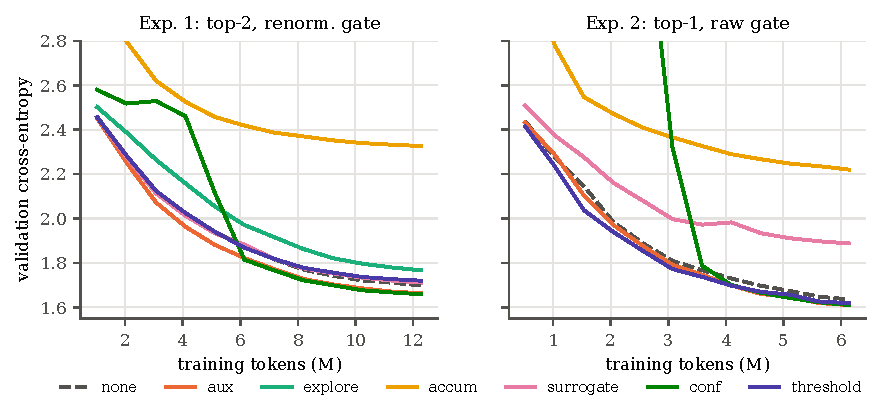
\includegraphics[width=\linewidth]{figures/val_loss.pdf}
\caption{Validation loss against training tokens. \code{conf} stays near 2.5 while it routes densely and evaluation (always top-$k$) does not match training, then drops sharply as its threshold anneals. \code{accum} is undertrained at equal tokens, taking one-eighth of the optimiser steps.}
\label{fig:loss}
\end{figure}

\subsection{Exp.~3: equal optimiser steps}
\label{sec:exp3}
\Cref{tab:exp3} shows the results of Exp.~3. Given equal updates, accumulation's hypothesis holds: loss 1.884 against 2.166, $\Hn$ 0.989 against 0.962, dropping 6.5\% against 17.0\%. It is, however, the least compute-efficient: 156.3 TFLOPs to reach 1.884, whereas \code{aux} in Exp.~1 reaches 1.663 on 63.6 TFLOPs. Its advantage is per update, which matters only when updates rather than FLOPs are scarce.

\begin{table}[htbp]
\centering
\caption{\textbf{Exp.~3} (as Exp.~1, but 1{,}000 optimiser steps for every strategy).}
\label{tab:exp3}
\small
\begin{tabular}{lcccccc}
\toprule
strategy & val loss $\downarrow$ & $\Hn\uparrow$ & max load $\downarrow$ & dropped $\downarrow$ & TFLOPs & tokens \\
\midrule
\code{accum}     & \textbf{1.884} & 0.989 & 0.167 & 6.49\% & 156.3 & 32.8M \\
\code{aux}       & 2.105 & \textbf{0.998} & \textbf{0.137} & \textbf{0.17\%} & 21.1 & 4.1M \\
\code{conf}      & 2.128 & 0.991 & 0.167 & 6.64\% & 33.0 & 4.1M \\
control          & 2.166 & 0.962 & 0.207 & 17.01\% & 18.4 & 4.1M \\
\code{threshold} & 2.173 & 0.992 & 0.177 & 11.52\% & 18.1 & 4.1M \\
\code{surrogate} & 2.178 & 0.981 & 0.184 & 20.45\% & 18.0 & 4.1M \\
\code{explore}   & 2.183 & 0.988 & 0.178 & 5.18\% & 20.5 & 4.1M \\
\bottomrule
\end{tabular}
\end{table}

\begin{figure}[t]
\centering
\begin{minipage}[t]{0.48\linewidth}
  \centering
  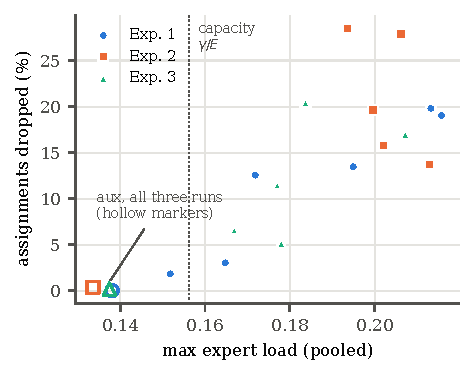
\includegraphics[width=\linewidth]{figures/maxload_vs_drop.pdf}
  \caption{Pooled max load against dropped assignments for every run; hollow markers are \code{aux}. Dropping rises with the busiest expert's share relative to the capacity line $\gamma/E=0.156$, but pooled max load is only a loose predictor, because capacity is enforced per layer and per batch.}
  \label{fig:maxload}
\end{minipage}\hfill
\begin{minipage}[t]{0.48\linewidth}
  \centering
  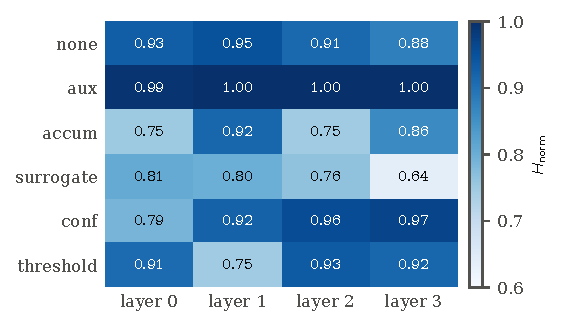
\includegraphics[width=\linewidth]{figures/per_layer_entropy.pdf}
  \caption{Per-layer $\Hn$ in Exp.~2. Pooled $\Hn$ for \code{surrogate} is a healthy-looking 0.965 while its last layer has collapsed to 0.640.}
  \label{fig:layers}
\end{minipage}
\end{figure}

\FloatBarrier
\subsection{Cross-cutting findings}
\label{sec:cross}

\paragraph{Max load predicts dropping; entropy saturates.} Across all runs $\Hn$ lies between 0.958 and 1.000 and barely discriminates, while dropping tracks the busiest expert's share against the capacity line almost exactly in Exp.~1 (\cref{fig:maxload}). Max load is the operationally meaningful collapse metric.

\paragraph{Pooling hides collapse.} Every run reports zero dead experts when pooled over layers; per layer, the same runs lose up to eleven. Model-level averages are not collapse diagnostics.

\paragraph{A capacity factor is itself an anti-collapse force.} Re-running Exp.~3 without a capacity limit, \code{accum}'s advantage in $\Hn$ over the control vanished (0.973 vs 0.970, against 0.989 vs 0.962 with the limit) and \code{threshold}'s entropy declined monotonically through training (0.963$\to$0.930), the only strategy to do so. Dropping lowest-gate-first denies an overloaded expert its marginal tokens and therefore its marginal gradient.

\paragraph{None of the metrics measure specialisation.} Every quantity above is a function of the load histogram. As \cref{sec:balance-spec} explains, the \code{aux} router's $\Hn=0.999$ is consistent with a well-specialised partition and with near-random routing alike. The experiments show which strategies prevent collapse; they say nothing about which produce experts.

% ===========================================================================
\section{Discussion}
\label{sec:discussion}

At this scale the auxiliary loss is the strongest single method on every axis we measured, and it is untuned. The alternatives that use no auxiliary loss each contribute a mechanism that works somewhere: \code{conf} matches or beats the auxiliary loss on quality without any balancing loss, paying extra only during training, although we cannot yet say whether its per-token confidence rule adds anything over a plain dense warm-up; \code{surrogate} shows that dense router gradients help when they are the router's only signal; \code{accum} shows that lower-variance router updates reduce collapse; \code{explore} lowers the load on the busiest experts, which sharply cuts dropped assignments; and \code{threshold} shows that the number of experts needed per token is often much less than $k$. Each is also worse than doing nothing in at least one setting: on quality for all except \code{conf}, which beats the control on validation loss everywhere but leaves the router less balanced in Exp.~1.

We read these results as consistent with the paper's premise rather than as evidence against it. The auxiliary loss is best at the one thing it optimises, an even spread of load, and that is all our metrics measure. Whether any of these methods produces the specialisation that \cref{hyp:shrink} requires is exactly the question the pilot could not answer. The literature is suggestive but not conclusive. Hash and random routing are competitive with learned routing \citep{roller2021hash,zuo2022thor,fan2024empirical}, Mixtral shows weak domain specialisation \citep{jiang2024mixtral}, and expert activations in deeper layers are near-identical across semantically unrelated inputs, especially in reasoning models \citep{wang2026myth}. Together these suggest that current learned routers are closer to balanced hashes than to partitions. Relaxing the \emph{scope} of balancing from micro-batch to global batch produces clearly more specialised experts and better models \citep{qiu2025demons}, and decoupling balancing from the gradient improves quality \citep{wang2024auxfree}, which suggests that the balancing term actively suppresses specialisation that the task gradient would otherwise produce.

The random-routing results also admit a reading that cuts against our hypothesis. Random routing may match learned routing because experts at current sizes are large enough to handle any mix of tokens, in which case how tokens are partitioned does not matter much and better routing would not let experts shrink. \citet{zuo2022thor} also observe near-random gating both with and without a load-balancing loss, so the balancing loss is unlikely to be the only reason routers fail to specialise. None of these studies varies expert size, so none can separate the two readings. The shrinkage experiment (\cref{sec:shrinkage}) is designed to do exactly that: our hypothesis predicts that specialised routing pulls ahead of random routing as experts shrink, while the alternative predicts that it does not.

\subsection{Limitations}
\label{sec:limitations}
All results come from one seed, one 2.4M-parameter model, one small homogeneous character-level corpus, and at most 3{,}000 optimiser steps per run. Quality differences of a few percent of perplexity are not significant. Hyper-parameters of every strategy, including $\alpha$, are untuned. We measure balance, not specialisation, and the shrinkage hypothesis is argued, not demonstrated. Compute is reported analytically and excludes dispatch overheads that matter in practice. Our argument in \cref{sec:balance-spec} concerns the routers that minimise the loss; it does not claim that auxiliary-loss training \emph{converges} to random routing, only that the loss provides no pressure away from it.

% ===========================================================================
\section{A protocol for testing specialisation and shrinkage}
\label{sec:protocol}

We describe the experiment we would run with adequate compute. Its purpose is to test \cref{hyp:shrink} directly and to rank strategies on specialisation, not only on balance.

\subsection{Scale and data}
\begin{itemize}
  \item \textbf{Tokenisation and corpus.} Subword tokens on a large, \emph{domain-labelled} mixture (e.g.\ web text, code, mathematics, several natural languages), so that specialisation has something to latch onto and can be measured against ground-truth domains. Character-level Shakespeare is too homogeneous for domain specialisation to exist.
  \item \textbf{Two model scales.} A sweep scale of roughly 100--150M active parameters trained near the compute-optimal token count \citep{hoffmann2022training} ($\sim$2--3B tokens), and a confirmation scale of about 1B active parameters for the best three configurations. Collapse and specialisation are both known to change with scale and training length, and our 3{,}000-step runs are far from either regime.
  \item \textbf{More and finer experts.} $E\in\{8,32,64\}$ with $k\in\{1,2,8\}$, including a fine-grained configuration with shared experts \citep{dai2024deepseekmoe}.
  \item \textbf{Seeds.} At least three per configuration, reporting mean and standard deviation; single-seed rankings in our tables should not be trusted.
\end{itemize}

\subsection{Baselines}
In addition to our seven configurations: global-batch auxiliary loss \citep{qiu2025demons}; auxiliary-loss-free bias balancing \citep{wang2024auxfree}; Default MoE dense backpropagation \citep{panda2025dense}; expert-choice routing \citep{zhou2022expertchoice}; a frozen random-hash router \citep{roller2021hash}, which is the \emph{null model for specialisation}: any method whose specialisation metrics do not beat it has not learned to route; and a dense model of equal active parameters.

\subsection{Specialisation metrics}
All computed per layer on held-out data:
\begin{enumerate}
  \item \textbf{Token--expert mutual information} $I(X;\mathcal{E})$ from \eqref{eq:mi}, split into its balance and per-token-entropy terms, normalised by $\ln E$.
  \item \textbf{Domain--expert mutual information} $I(D;\mathcal{E})$ \citep{gu2025elasticmoe} using the corpus's domain labels, together with per-domain dispatch histograms in the style of \citet{muennighoff2025olmoe}.
  \item \textbf{Routing stability}: the fraction of held-out tokens routed to the same top-1 expert at checkpoint $s$ and at the final checkpoint, which separates a stable partition from high-entropy churn \citep{dai2022stablemoe}.
  \item \textbf{Functional specialisation}: the increase in loss when expert $i$ is removed \citep{engmann2026causal}, measured separately on each domain. \citet{dai2024deepseekmoe} use a related test, disabling the top routed experts to measure redundancy. A specialised expert has a large, domain-concentrated ablation effect; a redundant one has a small, uniform effect.
  \item \textbf{Expert redundancy}: mean pairwise linear CKA \citep{kornblith2019similarity} between experts' outputs on a common probe set of inputs. Redundant generalists have high CKA; \cref{hyp:shrink} predicts that CKA falls as $I(X;\mathcal{E})$ rises.
  \item \textbf{Collapse metrics} as in this paper, always per layer, with max load reported alongside $\Hn$.
\end{enumerate}

\subsection{The shrinkage experiment}
\label{sec:shrinkage}
The decisive test of \cref{hyp:shrink}. For each routing procedure $\mathcal{R}$, train models whose expert width is $d_h/r$ for $r\in\{1,2,4,8\}$, holding $E$, $k$, the backbone and the token budget fixed, and plot validation loss against total expert parameters $E\,d_h/r$. The hypothesis predicts that the loss-versus-memory curve is flatter for procedures with higher measured specialisation. Two complementary controls: (i) at fixed \emph{active} compute, reduce $E$ instead of $d_h$, to separate ``fewer experts'' from ``smaller experts''; and (ii) apply post-hoc merging \citep{li2024mcsmoe} and pruning \citep{lu2024notall} to the $r=1$ models, measuring how much each procedure's experts can be compressed after training. If specialised routing yields experts that compress \emph{less} post hoc but can be trained \emph{smaller} a priori, that is strong evidence for the hypothesis.

\subsection{Ablations that our pilot flagged}
\begin{itemize}
  \item Tune $\alpha$ for the auxiliary loss, including very small values: its dominance here is untuned.
  \item \code{explore} with a lower starting rate $\epsilon_0\in\{0.1,0.2,0.3\}$, since $0.6$ disrupts more than it helps, and a floor $\epsilon_1$ higher than the current $0.01$.
  \item A plain dense warm-up of 10--20\% of training, to isolate whether \code{conf}'s gains come from confidence gating or simply from dense early training.
  \item \code{surrogate} only with the renormalised gate, compared with Default MoE's per-expert estimate.
  \item With and without capacity factor, since the limit itself suppresses collapse.
\end{itemize}

\subsection{Compute estimate}
Using the $6ND$ approximation \citep{kaplan2020scaling} with $N$ active parameters, a 125M-active model trained on 2.5B tokens costs about $1.9\times10^{18}$ FLOPs; at an effective $10^{14}$~FLOP/s on one A100 (roughly 30\% utilisation, discounted further for MoE dispatch overhead), that is about 5--10 GPU-hours per run. The sweep (ten routing procedures, four expert widths, three seeds) is 120 runs, or on the order of 1{,}000 GPU-hours. The confirmation scale ($\sim$1B active parameters, 20B tokens, $\sim1.2\times10^{20}$ FLOPs per run) for three configurations and two seeds adds on the order of 2{,}000 GPU-hours. The full protocol is therefore in the low thousands of A100-hours: modest for an industrial lab, well beyond the budget used for the pilot.

\subsection{Toward a combined method}
\label{sec:combined}
No single strategy we tested produces routers that are both balanced and specialised, and we do not expect one to. A method that gets experts to specialise properly will most likely need to combine several of the strategies covered here, and possibly others we have not tested, such as an explicit reward for decisive routing. Designing that combination is the natural next step once the protocol above can measure specialisation.

% ===========================================================================
\section{Conclusion}
Preventing router collapse and producing specialised experts are different objectives. The standard auxiliary loss is an effective answer to the first, and in our pilot the most effective one, but it is provably indifferent to the second. Specialisation is what would let each expert be smaller and would attack the memory cost that defines MoE deployment. We have described six mechanisms for preventing collapse, characterised where each helps and fails, argued that getting experts to specialise will likely require combining several of them, and set out the experiment that would test whether specialised routers really allow smaller experts. The code for every experiment in this paper is available at \url{https://github.com/muadmazahir/MoE-experiments}, so that the protocol can be run by anyone with the compute to do so.

\bibliographystyle{plainnat}
\bibliography{refs}

% ===========================================================================
\clearpage
\appendix
\section{Hyper-parameters}
\Cref{tab:train} lists the settings shared by every run and \cref{tab:hparams} the defaults for each strategy. $S$ is the total number of training steps.

\begin{table}[H]
\centering
\caption{Model and training settings shared by every run. Where Exp.~2 differs, its value is given in brackets.}
\label{tab:train}
\small
\begin{tabular}{ll}
\toprule
setting & value \\
\midrule
layers, width $d$, heads, context & 4, 128, 4, 128 \\
experts $E$, experts per token $k$ & 8, 2 (1) \\
expert hidden width $d_h$ & 256 \\
gate & renormalised (raw) \\
dropout & 0 \\
optimiser & AdamW, $\beta=(0.9,\,0.95)$ \\
learning rate & $3\times10^{-4}$ ($10^{-3}$) \\
schedule & 5\% linear warm-up, cosine decay to 10\% \\
weight decay & 0.1, on weight matrices only \\
gradient clipping & 1.0 (global norm) \\
batch size & 32 (16) sequences of 128 characters \\
training steps & 3{,}000 (Exp.~3: 1{,}000 optimiser steps) \\
evaluation & every 250 steps, on 20 fixed held-out batches \\
seed & 0 \\
\bottomrule
\end{tabular}
\end{table}

\begin{table}[H]
\centering
\caption{Default strategy hyper-parameters.}
\label{tab:hparams}
\small
\begin{tabular}{lll}
\toprule
strategy & hyper-parameter & value \\
\midrule
\code{aux} & loss weight $\alpha$ & $10^{-2}$ \\
\code{explore} & $\epsilon_0\to\epsilon_1$, anneal fraction $\rho$ & $0.6\to0.01$, $0.6S$ \\
 & gate temperature $T$ (exploring tokens only) & 4 (constant) \\
\code{accum} & micro-batches per step $M$ & 8 \\
\code{surrogate} & straight-through weight $\alpha_s$ & 1.0 \\
\code{conf} & $\tau_c^0$, annealed to 0 over & 0.8, $0.8S$ \\
\code{threshold} & $\tau_0\to\tau_1$ (units of $1/E$), rise over & $1.0\to1.6$, $0.8S$ \\
all & capacity factor $\gamma$ & 1.25 \\
\bottomrule
\end{tabular}
\end{table}

\section{Reproducing the experiments}
The code is available at \url{https://github.com/muadmazahir/MoE-experiments}. From the repository root, the three experiments and the figures are reproduced with:
\begin{small}
\begin{verbatim}
# Exp. 1: top-2, renormalised gate, equal tokens
python run_experiment.py --steps 3000 --capacity-factor 1.25 \
    --seeds 0 --out results/exp1-seed0
# Exp. 2: top-1, raw gate
python run_experiment.py --k 1 --gate-norm raw --capacity-factor 1.25 \
    --lr 1e-3 --batch-size 16 --steps 3000 \
    --methods none,aux,accum,surrogate,conf,threshold \
    --seeds 0 --out results/exp2-seed0
# Exp. 3: equal optimiser steps
python run_experiment.py --equalize steps --steps 1000 --capacity-factor 1.25 \
    --seeds 0 --out results/exp3-seed0
# Figures
python paper/figures/make_figures.py
\end{verbatim}
\end{small}

\end{document}
